
To provide an overview of all the topics that will be addressed, we will begin by defining the key components of this thesis and explaining the basics to build upon in the later chapters. 

\section{Web Applications}
\label{sec:webapp}
A \textit{web application} has been defined as “a software application, executed by a web server, which responds to dynamic web page requests over HTTP” by the Web Application Security Consortium \gls{wasc}~\cite{noauthor_web_2012}. 
In simpler terms, a web application is software that runs on a server and users access it through a web browser (like Chrome or Firefox) over the internet.

Typically, the resources and scripts of web applications — such as images, text, or functionalities — are requested by the client, which is the user's computer or device, using a web browser or similar tools. This interaction follows a set of rules known as the \gls{api}, which specifies what requests can be made and how the server should respond.
The~\autoref{fig:simplified-web-app} illustrates the basic communication process between the client (the user's device), the server (where the application runs), and external services (such as another server).

Most web applications also use a database, which is a structured way of storing data, to keep information consistently available and reliable. For the purposes of this thesis, we assume that the web application has a monolithic architecture. This means that it operates as a single cohesive program on a physical computer, rather than being divided into separate parts that run on different cloud services (like AWS, or Amazon Web Services, which offers online computing power without needing dedicated hardware\footnote{https://aws.amazon.com/})
Additionally, we assume the server follows \gls{rest} principles, which are guidelines for how web services should operate to enable smooth communication as described by \citet{roy_t_fielding_rest_2008}. 
The web server processes requests that adhere to the \gls{http} standard, which is the foundational protocol used for transmitting data on the web (ref. ~\autoref{tab:rest_http_methods}). It can be used  with the database operations, commonly known as \gls{crud} operations, as established by \citet{martin_managing_1983}, when a web application utilizes a persistent database.
This adherence ensures that the server and client can operate independently, meaning they can be developed and updated separately without affecting each other\cite{fielding_http_2022}.


\begin{figure}[ht]
    \centering
    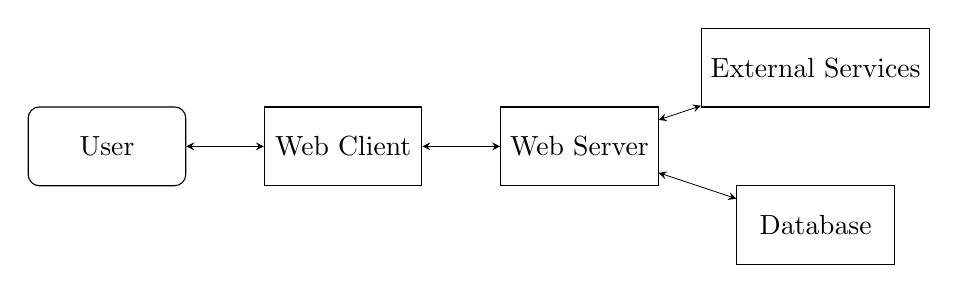
\begin{tikzpicture}[node distance=3cm]
    % Define styles for nodes and arrows
    \tikzstyle{user} = [rectangle, rounded corners, minimum width=2cm, minimum height=1cm, text centered, draw=black]
    \tikzstyle{browser} = [rectangle, minimum width=2cm, minimum height=1cm, text centered, draw=black]
    \tikzstyle{server} = [rectangle, minimum width=2cm, minimum height=1cm, text centered, draw=black]
    \tikzstyle{database} = [rectangle, minimum width=2cm, minimum height=1cm, text centered, draw=black]
    \tikzstyle{external} = [rectangle, minimum width=2cm, minimum height=1cm, text centered, draw=black]
    % Use arrows with both directions
    \tikzstyle{arrow} = [thick, <->, >=stealth]
% Arrow style for double lines

    \tikzset{doubleArrow/.style={thick, <->, >=stealth,
        line width=0.1mm, line cap=round, draw=black
    }}
    % Nodes
    \node (user) [user] {User};
    \node (browser) [browser, right of=user] {Web Client};
    \node (server) [server, right of=browser] {Web Server};
    \node (database) [database, right of=server, yshift=-1cm] {Database};
    \node (external) [external, right of=server, yshift=1cm] {External Services};
    % Arrows (connections)
    \draw  [doubleArrow](user) -- (browser);
    \draw  [doubleArrow](browser) -- (server);
    \draw  [doubleArrow](server) -- (database);
    \draw [doubleArrow] (server) -- (external);
    \end{tikzpicture}
    \caption{Structure of a simplified Web Application}
    \label{fig:simplified-web-app}

\end{figure}

\begin{table}[htb]
    \centering
    \begin{tabular}{@{}lll@{}}
        \toprule
        \textbf{HTTP Method} & \textbf{Purpose}                         & \textbf{Idempotent} \\ \midrule
        GET                   & Retrieve a resource                     & Yes                 \\
        POST                  & Create a new resource                   & No                  \\
        PUT                   & Update or create a resource             & Yes                 \\
        PATCH                 & Partially update a resource             & Yes (mostly)        \\
        HEAD                  & Retrieve headers of a resource         & Yes                 \\
        OPTIONS               & Return available HTTP methods           & Yes                 \\
        DELETE                & Remove a resource                       & Yes                 \\ \bottomrule
    \end{tabular}
    \caption[List of HTTP Methods]{Summary of REST HTTP Methods and their idempotence \cite[chapter 9]{fielding_http_2022}}
    \label{tab:rest_http_methods}
\end{table}
\FloatBarrier

\section{Cross-Site Scripting}
\label{sec:xss}
\textit{Cross-site scripting} (XSS) is a security vulnerability that enables the execution of malicious code on a remote server or
another client by exploiting weaknesses in server-side input validation. \cite{bisht_xss-guard_2008}
According to the Open Web Application Security Project (OWASP) top 10 list, XSS, and other code injection techniques, are the second most common vulnerabilities in web applications, only surpassed by broken access control.\cite{noauthor_owasp_2025}

\citet{tang_identifying_2012} describe two kinds of XSS attacks, reflected, or non-persistent, XSS and persistent XSS.
\subsection{Reflected XSS}

Reflected XSS means, 


\subsection{Persistent XSS}

\autoref{fig:xss-simp} illustrates a simplified scenario in which persistent XSS can be employed to execute code on
another machine by sending malicious code to the server, which subsequently transfers this malicious code to unsuspecting clients.
A common instance of this vulnerability occurs when an application provides a web interface that allows users
to enter and store text without adequate server-side input validation and sanitization,
thereby failing to prevent users from executing HTML scripts on the devices of other users.

A recent example of this would be a vulnerability in the web interface web UI of Cisco Enterprise Chat and 
Email\footnote{https://www.cisco.com/c/en/us/support/docs/csa/cisco-sa-ece-xss-CSQxgxfM.html}. 
Cisco is a company that develops communication and security-related tools, 
underscoring the critical need for rigorous testing for vulnerabilities,
as even organizations specializing in security can overlook certain issues.

The severity of a vulnerability hinges on the accessibility of the exploit. 
If an attack requires authentication and allows for traceability,
it may represent a minor inconvenience and therefore calls for a patch of the issue,
as the attacker can be identified. However, if an XSS attack can be executed anonymously,
this poses a significant risk to all users and requires immediate remediation.


%\clearpage
\begin{figure}[H]
\centering
\begin{adjustbox}{height=5cm}
\begin{tikzpicture}[node distance=1cm]

\tikzstyle{startstop} = [rectangle, rounded corners, minimum width=3cm, minimum height=1cm,text centered, draw=black, fill=red!30]

\tikzstyle{process} = [rectangle, minimum width=3cm, minimum height=1cm,text centered, draw=black, fill=orange!30]
\tikzstyle{decision} = [diamond, minimum width=3cm, minimum height=1cm, text centered, draw=black, fill=lmugreen!69]
\tikzstyle{arrow} = [thick,->,>=stealth]



\node (start) [startstop] {Malicious Attacker Client};
\node (pro1) [process, below = of start] {\lstinline{ <script>alert("Hello")</script>}};
\node (dec1) [decision, below = of pro1] {Server};
\node (pro2a) [startstop, below  = of dec1, xshift=-3cm] {Unassuming Client};
\node (pro2b) [startstop, below  = of dec1, xshift=3cm] {Unassuming Client};
\node (stopA) [process, below = of pro2a] {Hello};
\node (stopB) [process, below = of pro2b] {Hello};


\draw  [arrow](start) -- node[anchor=east] {post message} (pro1);
\draw  [arrow](pro1) -- node[anchor=east] {store message}(dec1);
\draw  [arrow](dec1) -- node[anchor=east] {distribute message} (pro2a);
\draw [arrow] (dec1) -- node[anchor=west] {distribute message} (pro2b);
\draw [arrow] (pro2a) -- node[anchor=west] {execute code}(stopA);
\draw [arrow] (pro2b) -- node[anchor=west] {execute code}(stopB);
\end{tikzpicture}
\end{adjustbox}      
    \caption[Simplified XSS attack example]{An example of a XSS attack. A malicious attacker sends a message to the server that contains a script, which will be distributed to clients. Upon receiving the message, the script will be executed.}
    \label{fig:xss-simp}
\end{figure}


\section{Testing}
The next aspect we would like to concentrate on is the testing of a web application. First we define what “testing” means, then look into the methodology of “fuzzing” as a technique used to test.

At its essence, \textit{testing} constitutes the systematic process of validating and verifying the functionality of a program. A sensible analogy for the concepts of validation and verification was articulated by \citet{b_w_boehm_verifying_1984}:

\begin{itemize}[label={}]
    \item \textit{Verification}: “Am I building the product right?” 
    \item \textit{Validation}: “Am I building the right product?”
\end{itemize}
Depending on the nature of the testing methodology employed, different levels of  assessment can be achieved. A unit test, which is designed to evaluate a single component or function—hence the term “unit”—primarily provides insights into the correctness of that individual function. \cite{beck_test-driven_2003}

In contrast, an end-to-end test, while potentially less precise in verifying the functionality of individual components, serves to validate the overall functionality of the entire system, with all components integrated. \cite{paul_end--end_2001}

Given that a program can accommodate a vast array of potential inputs, it may be impractical to manually identify all possible variations. Therefore, we can utilize a technique known as “fuzzing”.

\section{Fuzzing}
\label{sec:fuzzing}
\textit{Fuzzing} is an automated process that involves the generation of input data to identify potential program errors, commonly referred to as “bugs”, which may arise from unhandled cases. These cases can include scenarios such as incompatible data types, excessively large entities, or the presence of unexpected characters.
The most basic idea of fuzzing is generating random input strings, which, when it was done first, already found bugs and crashes in the tested libraries \cite{miller_empirical_1990}.\\
Fuzzing can be done in different ways, and in the following we will describe the two most commonly used types: “white-box” fuzzing and “black-box” fuzzing.


\vspace{0.5cm}
\begin{tabular*}{\textwidth}{@{}c|c@{}}
    
\begin{minipage}{\dimexpr0.5\textwidth-2\tabcolsep}
\centering
    % Left Diagram - White Box Fuzzing
    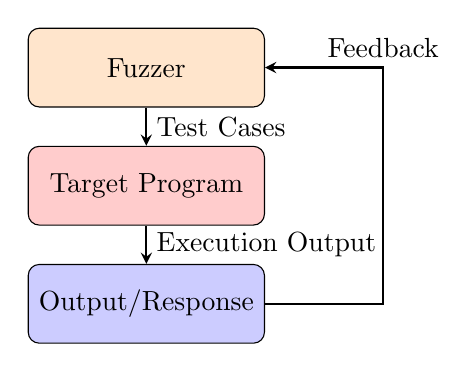
\begin{tikzpicture}[node distance=1.5cm]
                % Define styles for nodes and arrows
        \tikzstyle{box} = [rectangle, rounded corners, minimum width=3cm, minimum height=1cm, text centered, draw=black, fill=blue!20]
        \tikzstyle{fuzzer} = [rectangle, rounded corners, minimum width=3cm, minimum height=1cm, text centered, draw=black, fill=orange!20]
        \tikzstyle{target} = [rectangle, rounded corners, minimum width=3cm, minimum height=1cm, text centered, draw=black, fill=red!20]
        \tikzstyle{arrow} = [thick,->, >=stealth]
        \tikzstyle{title} = [rectangle, rounded corners, minimum width=5cm, text centered, draw=none, fill=none, font=\large\bfseries] 
    
        \node (fuzzer) [fuzzer] {Fuzzer};
        \node (target) [target, below of = fuzzer] {Target Program};
        \node (output) [box, below of = target] {Output/Response};

        % Arrows
        \draw  [arrow](fuzzer) -- (target) node[midway, right] {Test Cases};
        \draw [arrow] (target) -- (output) node[midway,right] {Execution Output};
        \draw [arrow] (output.east) --+(1.5,0) |- (fuzzer.east) node[midway, above] {Feedback};
    \end{tikzpicture}

\end{minipage}
&
\begin{minipage}{\dimexpr0.5\textwidth-2\tabcolsep}
\centering

    % Left Diagram - White Box Fuzzing
    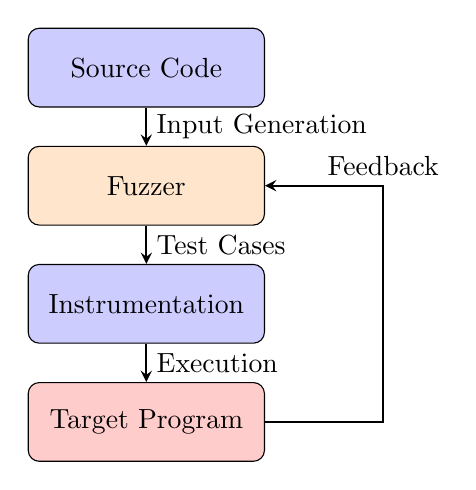
\begin{tikzpicture}[node distance=1.5cm]

        \tikzstyle{box} = [rectangle, rounded corners, minimum width=3cm, minimum height=1cm, text centered, draw=black, fill=blue!20]
        \tikzstyle{fuzzer} = [rectangle, rounded corners, minimum width=3cm, minimum height=1cm, text centered, draw=black, fill=orange!20]
        \tikzstyle{target} = [rectangle, rounded corners, minimum width=3cm, minimum height=1cm, text centered, draw=black, fill=red!20]
        \tikzstyle{arrow} = [thick,->, >=stealth]
        \tikzstyle{title} = [rectangle, rounded corners, minimum width=5cm, text centered, draw=none, fill=none, font=\large\bfseries]
        \node (source) [box] {Source Code};
        \node (fuzzer) [fuzzer, below of = source] {Fuzzer};
        \node (instr) [box, below of = fuzzer] {Instrumentation};
        \node (target) [target, below of = instr] {Target Program};

        % Arrows
        \draw  [arrow](source) -- (fuzzer) node[midway, right] {Input Generation};
        \draw  [arrow](fuzzer) -- (instr) node[midway, right] {Test Cases};
        \draw  [arrow](instr) -- (target) node[midway, right] {Execution};
        \draw  [arrow](target.east) -- +(1.5,0) |- (fuzzer.east) node[midway, above] {Feedback};

    \end{tikzpicture}
    
\end{minipage}

\\

\begin{minipage}[t]{\dimexpr0.5\textwidth-1\tabcolsep}
\captionof{figure}{Simplified black-box fuzzing process}
    \label{fig:black-box-testing}

\end{minipage}
&
\begin{minipage}[t]{\dimexpr0.5\textwidth-1 \tabcolsep}
\captionof{figure}{Simplified white-box \\fuzzing process}
\label{fig:white-box-testing}

\end{minipage}

\end{tabular*}

\subsection{Black Box Fuzzing}
\label{sec:black-box}
\textit{Black box fuzzing} (ref. \autoref{fig:black-box-testing}) is a software testing method that evaluates an application’s security and robustness by feeding it random or semi-random inputs without any knowledge of its internal workings—such as source code, data structures, or algorithms. This approach simulates an external attacker's perspective, enabling testers to discover vulnerabilities that might be exploited by malicious users in a real-world scenario.

The key characteristic of black-box fuzzing is its lack of insight into the internal design and logic of the software being tested. Instead, the focus is on the inputs and outputs of the application. Testers generate a wide variety of input data, often using automated tools or scripts, to gauge how the application responds. This can include testing edge cases, invalid inputs, or unexpected data formats to determine how robust the application is against improper use.

One of the main advantages of black-box fuzzing is its simplicity and ease of use. Since testers do not need to understand the details of the application’s code, they can quickly implement fuzzing without extensive knowledge of the underlying logic. This makes black-box fuzzing an attractive option for assessing third-party software or legacy applications where source code is not available.

Black-box fuzzing can be effective in identifying common security vulnerabilities, such as buffer overflows, input validation errors, and unexpected crashes. By observing how the application behaves with various inputs, testers can pinpoint areas of insecurity, allowing developers to focus their remedial efforts on the most critical issues.

Though black-box fuzzing offers valuable insights into application security, it does have some limitations. Specifically, the randomness of the generated inputs might not exercise all potential execution paths, leaving some vulnerabilities undiscovered. Moreover, in the absence of an understanding of the internal code structure, it may prove challenging to determine which vulnerabilities are of greater significance based on their potential impact.
 \cite{godefroid_random_2007}

\subsection{White Box Fuzzing}
\label{sec:white-box}
\textit{White box fuzzing} (ref. \autoref{fig:white-box-testing}) is a software testing technique that seeks to identify vulnerabilities and bugs within applications by utilizing an in-depth understanding of their internal structures and logic. Unlike traditional black-box testing methods, where testers approach the software without any knowledge of its internal workings, white-box fuzzing leverages access to the source code, algorithms, and data flows, allowing for a more targeted and effective analysis.

One of the primary benefits of white-box fuzzing is its ability to generate test inputs based on the actual paths and branches present in the code. By analysing the control flow and data structures inherent to the application, a white-box fuzzer can create specific input cases that exercise various execution paths. This targeted approach increases the likelihood of uncovering potential weaknesses, particularly in areas of the code that may be prone to errors or security vulnerabilities.

Additionally, white-box fuzzing often incorporates dynamic analysis. More on that in ~\autoref{sec:dse}. During the fuzzing process, the application is executed in a controlled environment, and its behaviour monitored in real-time. This provides valuable feedback on how the program reacts to the generated inputs, enabling the identification of unhandled cases that may lead to crashes, incorrect outputs, or security flaws.

Another critical feature of white-box fuzzing is coverage measurement. By measuring code coverage, testers can ensure that their input generation strategies are effective in exercising different paths within the software. This helps identify areas of the code that have not been adequately tested, enabling a more comprehensive examination of the program's reliability and security.

The primary objective of white-box fuzzing is to detect issues such as buffer overflows, null pointer dereferences, and other runtime errors that could compromise an application’s stability or allow for security breaches. By identifying these vulnerabilities early in the development process, organizations can address them proactively, ultimately enhancing the overall quality and security of their software.\cite{godefroid_random_2007}




\section{Dynamic Symbolic Execution}
\label{sec:dse}
\textit{Dynamic symbolic execution} (DSE), first presented in the seventies \cite{boyer_selectformal_1975}\cite{king_new_1975}\cite{king_symbolic_1976}, is a form of white-box fuzzing, as it requires access to the source code. However, instead of generating all inputs from the start, it assumes that the variables are “symbolic”, meaning that they do not possess a tangible value during execution of the program. Instead, it tracks the conditions encountered during runtime, generating constraints based on the symbolic variables. 
This facilitates a comprehensive examination of multiple program pathways, thereby aiding in the identification of anomalies that may result in unforeseen behaviour or security vulnerabilities.
After exploring a particular execution path, DSE employs constraint solvers to analyse the constraints collected during execution. These solvers determine concrete inputs that can satisfy the path constraints, allowing the generation of specific test cases to trigger particular code paths during subsequent executions.

By using DSE, testers can automatically generate test cases that reliably expose bugs or vulnerabilities, such as buffer overflows or access violations. This allows for a more exhaustive testing process that can reveal flaws that traditional fuzzing techniques might overlook.

The synergy between DSE and white-box fuzzing promotes automated test generation and increases the coverage of tested paths, ultimately improving the software's reliability and security. It provides developers with concrete inputs that reproduce identified vulnerabilities, facilitating debugging and remediation.



\subsection{Example Dynamic Symbolic Execution}
In this subsection, we will demonstrate the concept of DSE by employing the code in \autoref{lst:example-program}. 
To facilitate the process, we can first depict the program as a Control Flow Graph (\gls{cfg}) \autoref{fig:example-program-graph}. 
The CFG displays the conditions and transformations along its edges, with the vertices signifying the state of the program.
On entering  the program, we assume that the initial value of x=1 and y=0, just to tell the DSE Engine the types of the variables, and to give a starting point. 
\capstartfalse
\begin{center}
    We can denote this as a tuple of (pc, S(x), C(x)) 
    \begin{table}[ht]
        \begin{tabular}{lll}
            where & pc & the path condition \\
             & $S(x) \rightarrow X$& \specialcell[c]{the symbolic state of X,\\ i.e. the applied transformations on the initial value}\\
             & $C(x) \rightarrow 0$& the concrete value of x\\
        \end{tabular}
    \end{table}
\end{center} 
\capstarttrue
\vspace{0.5cm}

\begin{tabular*}{\textwidth}{@{}c|c@{}}
    
\begin{minipage}{\dimexpr0.5\textwidth-2\tabcolsep}
\centering
    % Left Diagram - White Box Fuzzing

\begin{lstlisting}[language=JavaScript, gobble=4, escapechar=@]
    function g(x, y) {
        if (x !== y){
            x += y
        }
        else {
            if (y > 8){
                y+=1
            }
        }
        x += 1
        if (x != 0 )
        { 
          if ( y != 0){
            x = y
          }
        }
    }
\end{lstlisting}
   
\end{minipage}
&
\begin{minipage}{\dimexpr0.5\textwidth-2\tabcolsep}
\centering
     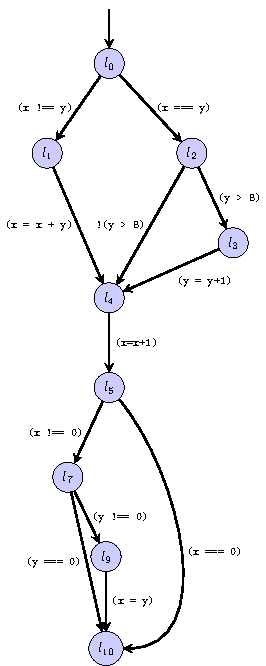
\includegraphics{../luatex/cfg/out/cfg.pdf}
\end{minipage}

\\

\begin{minipage}[t]{\dimexpr0.5\textwidth-1\tabcolsep}
 \captionof{lstlisting}{A simple program}
\label{lst:example-program}

\end{minipage}
&
\begin{minipage}[t]{\dimexpr0.5\textwidth-1 \tabcolsep}
\captionof{figure}{CFG of \autoref{lst:example-program}}
\label{fig:example-program-graph}

\end{minipage}

\end{tabular*}


In similar fashion, we can now walk through the execution, and create a branch whenever we encounter diverging paths.
For example, right at the start, we have two possible routes the execution can take: $x == y$ and $\neg(x == y)$.
We can now construct the symbolic execution tree displayed in \autoref{fig:symbolic-execution-tree} by tracking the path conditions and transformations of the variables.

\begin{sidewaysfigure}[h]
  \centering
  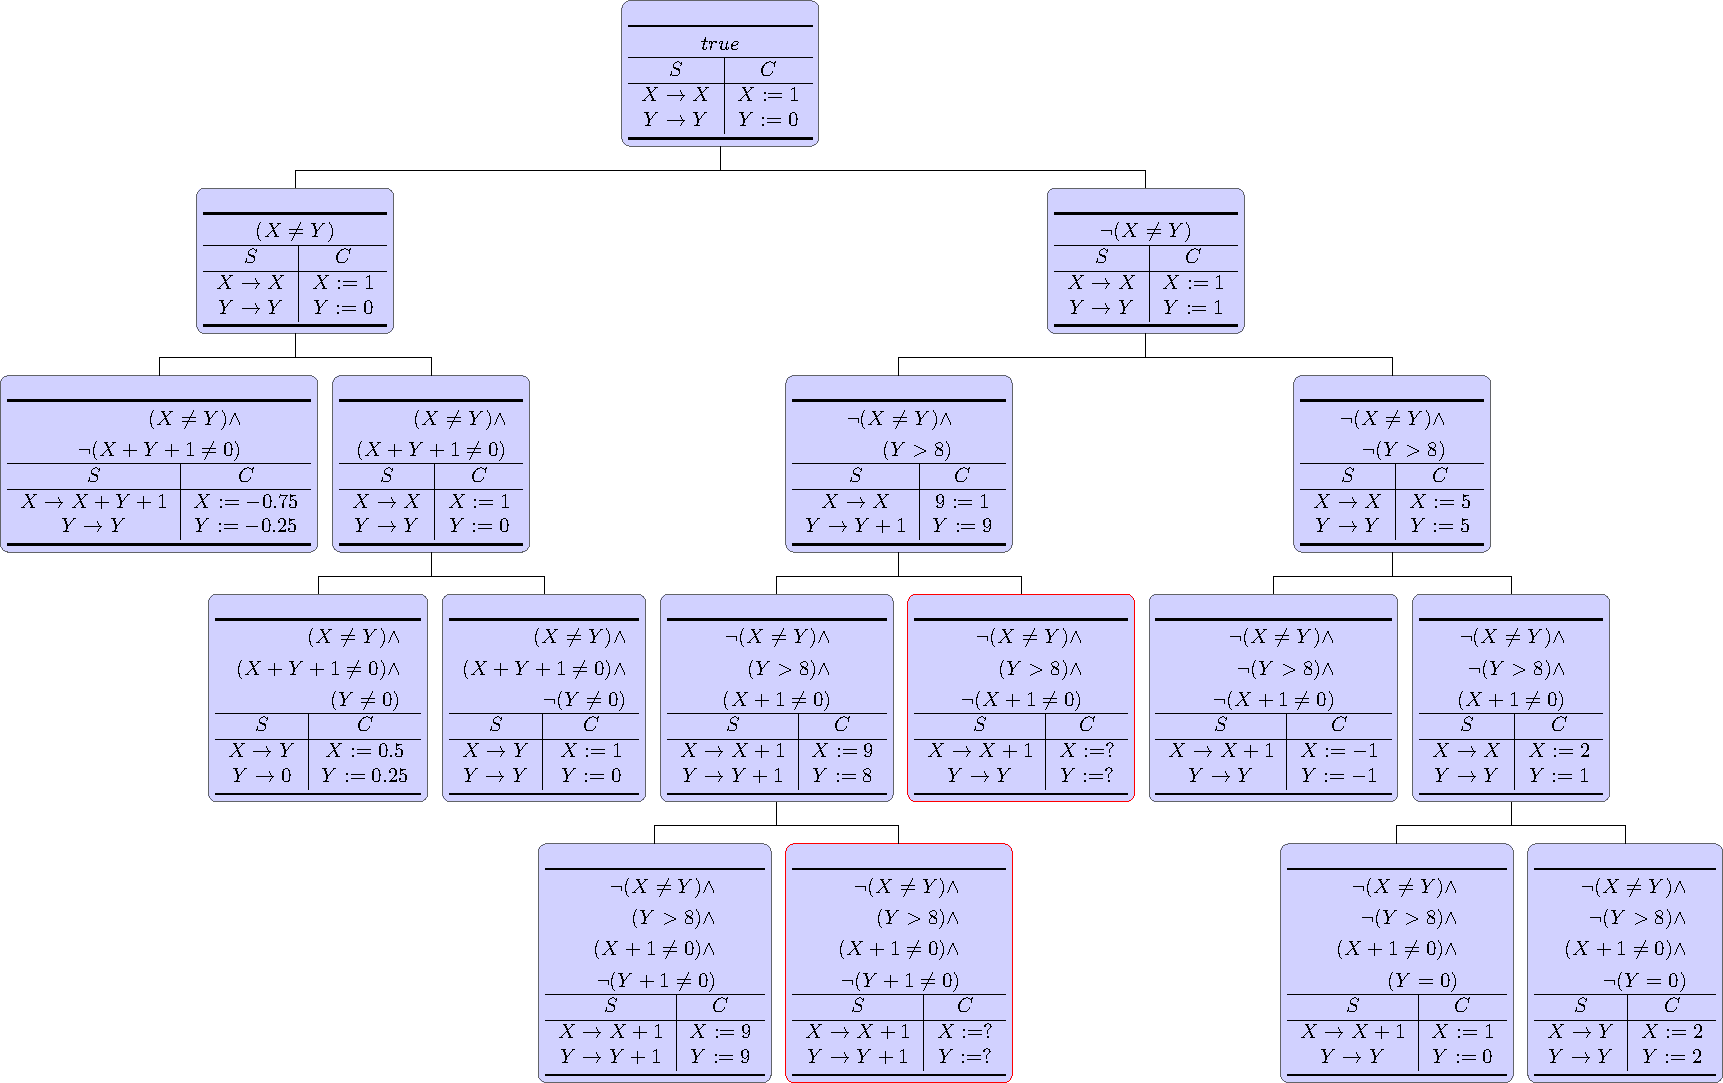
\includegraphics[width=\textwidth]{../luatex/symexe/out/symexe.pdf}    
  \caption[Symbolic execution tree]{Symbolic execution tree of \autoref{lst:example-program}, displaying the path condition and the concolic state. Unreachable paths are highlighted in red.}
  \label{fig:symbolic-execution-tree}
\end{sidewaysfigure}




After constructing the execution tree, we can generate distinct inputs for each of the leaf nodes, checking for satisfiability.
For instance, if we want to determine which input would cover the branch in the middle of the tree, we can do so by solving the constraints  $(\neg(X \neq Y) \land (Y > 8) \land \neg( X+1==0 ) \land \neg(Y+1 \neq 0 ))$. 
Solving these constraints yields the answer of (x = 9, y = 9), which indicates that this input will satisfy the specified conditions for that branch. 
Any condition that cannot be satisfied means that the leaf node cannot be reached, no matter the input. The two leafs highlighted in red in  \autoref{fig:symbolic-execution-tree} showcase this.
These constraints are usually solved by an SMT Solver, which we will briefly explain in \autoref{sec:z3}.


JavaScript has a few peculiarities, as it is dynamically typed and therefore only resolved at runtime. 

\subsection{Limitations DSE}

As with any explorative system, DSE has limitations regarding its capabilities. 
The most significant limitation is computable paths, which have the potential to explode if the analysed program is not designed with DSE in mind, for instance, if it heavily relies on recursive calls. 
But even with DSE in mind, the paths grow exponentially with the number of conditionals in a program.  \cite{cadar_symbolic_2013}
This also occurs with symbolic addresses, as it has to account for any possible memory address a variable can occupy \cite{elkarablieh_precise_2009}.  

To address this, most DSE frameworks employ various kinds of techniques for reducing the number of paths. 
One such technique is path merging based on heuristics, where a reoccurring conditional, can be merged into one (for example in a loop).\cite{kuznetsov_efficient_nodate}

\citet{cha_unleashing_2012} propose a solution for a symbolic memory, reducing the possible paths for symbolic addresses by concretizing writes and only allowing symbolic.    

It also is not suitable for full boundary testing, as DSE checks for reachability, and once a path is covered, it will not move back and check for edge case in this path, possibly missing unexpected behaviour, i.e. catching an integer overflow.\cite{berthier_efficient_2023}




